\ProvidesPackage{commands}
\documentclass[11pt]{article}
\usepackage{epstopdf}
\usepackage{subfigure,graphicx}
\usepackage{amsmath}
\usepackage{epsf}
\usepackage{amsfonts}
\usepackage{amssymb}
\usepackage{color}
\usepackage{mathtools}
\usepackage{placeins}
\usepackage{booktabs}
\usepackage{enumitem}
\usepackage{caption}
\usepackage[margin=0.8in, paperwidth=8.5in, paperheight=11in]{geometry}
\usepackage{amsfonts}
\usepackage{amsmath}
\usepackage{amsbsy}
\usepackage{authblk}
\usepackage{graphicx}
\usepackage{listings}
\usepackage{array}
\usepackage{titlesec}
\usepackage{amssymb}
\usepackage{bm}
\usepackage{mathtools}
\usepackage{titlesec}

\usepackage[latin1]{inputenc}\newcommand{\bs}[1]{\boldsymbol{#1}}
\newcommand{\del}[2]{\frac{\partial {#1}}{\partial {#2}}}
\newcommand{\D}[2]{\frac{D^{\overline{\alpha}}}{\overline{\alpha !}}{#1}(#2,#2)\ {\bf x}^{\overline{\alpha}}}
\newcommand{\dv}[3]{\frac{{\rm d}^{#1}{#2}}{d{#3}^{#1}}}
\newcommand{\ddel}[5]{\frac{\partial^{ {#1} + {#2}} {#3}}{\partial {#4}^{#1} \partial{#5}^{#2}}}
\newcommand{\dev}{{\rm {\bf dev}}}
\newcommand{\proj}[1]{\frac{1}{R^2}{\bf X}\otimes{\bf X}}
\newcommand{\Ie}[1]{I^{\rm e}_{#1}}
\newcommand{\Ce}[1]{\bf C^{\rm e^{#1}}}
\newcommand{\Fe}[2]{F^{\rm e^{#2}}_{#1}}
\newcommand{\Fv}[2]{F^{\rm v^{#2}}_{#1}}
\newcommand{\f}[2]{f^{\rm {#2}}_{#1}}
\newcommand{\fv}[2]{f^{\rm v^{#2}}_{#1}}
\newcommand{\dfv}[2]{\dot{f}^{\rm v^{#2}}_{#1}}
\newcommand{\tGam}[2]{\tilde{\Gamma}^{\rm v^{#2}}_{#1}}
\newcommand{\Gam}[2]{\Gamma^{\rm v^{#2}}_{#1}}
\newcommand{\A}[1]{\mathcal{A}_{#1}}
\newcommand{\F}[2]{F^{\rm #2}_{#1}}
\newcommand{\hpeq}{\hat{\psi}^{\rm Eq}}
\newcommand{\hpneq}{\hat{\psi}^{\rm NEq}}
\newcommand{\etak}{\eta_K({I_1,I_2,J},{\bf C^{\rm e}, B^{\rm v}})}
\newcommand{\nuk}{\nu_K({I_1,I_2,J},{\bf C^{\rm e}, B^{\rm v}})}
\newcommand{\thetak}{\theta_K({I_1,I_2,J},{\bf C^{\rm e}, B^{\rm v}})}
\newcommand{\etaj}{\eta_J({I_1,I_2,J},{\bf C^{\rm e}, B^{\rm v}})}
\newcommand{\dFv}[2]{\dot{F}^{\rm v^{#2}}_{#1}}
\newcommand{\hatpsi}{\widehat{\psi}(I_1, I_2,I^{\rm e}_1,I^{\rm e}_2,J)}
\newcommand{\hpsi}{\widehat{\psi}(I_1,I^{\rm e}_1,J)}
\newcommand{\Fh}[1]{\widehat{\mathcal{F}}\left({\bf F, \Fv{}{}}, {#1}\right)}
\newcommand{\Fhstar}[1]{\widehat{\mathcal{F}}^*\left({\bf F, \Fv{}{}}, {#1}\right)}
\newcommand{\sbar}{\overline{\bm{\sigma}}}
\newcommand{\hpsicomp}[1]{\sum_{r=1}^{2}\left\{\frac{3^{1-\alpha_r}}{2\alpha_r}\mu_r(I^{\alpha_r}_1-3^{\alpha_r})
+\frac{3^{1-a_r}}{2a_r}m_r({\Ie{1}}^{^{a_r}}-3^{a_r})\right\}
+\mu{#1}+\kappa{#1}^2}
\newcommand{\Ni}[1]{N^{(e)}_i(#1)}
\newcommand{\hNi}[1]{\hat{{N}}^{(e)}_i(#1)}
\newcommand{\Ld}{L^{\dagger}}
\newcommand{\intinfinf}{\int_{-\infty}^{\infty} \int_{-\infty}^{\infty}}
\newcommand{\LLnorm}[1]{\left\lVert{#1}\right\rVert_2}
\newcommand{\Linorm}[1]{{\left\lVert{#1}\right\rVert_\infty}}
\newcommand{\tr}{\rm tr}
\newcommand{\deldel}[2]{\frac{\partial^2 {#1}}{\partial {#2}^2}}
\newcommand{\kd}[1]{\delta_{#1}}



\titlespacing\section{10pt}{10pt plus 4pt minus 2pt}{10pt plus 2pt minus 2pt}
\titlespacing\subsection{0pt}{8pt plus 4pt minus 2pt}{8pt plus 2pt minus 2pt}
\titlespacing\subsubsection{0pt}{12pt plus 4pt minus 2pt}{6pt plus 2pt minus 2pt}
\titlespacing*{\title}{-2ex}{*-2ex}{-2ex}
\usepackage{color} %red, green, blue, yellow, cyan, magenta, black, white
\definecolor{mygreen}{RGB}{28,172,0} % color values Red, Green, Blue
\definecolor{mylilas}{RGB}{170,55,241}
\setlength\parindent{0pt}
\graphicspath{{/}}

\title{\bf CSE 401: Numerical Analysis \\ HW 7}
\author{Bhavesh Shrimali \\ NetID: bshrima2}
\date{\today}
\titlespacing*{\title}{-2ex}{*-2ex}{-2ex}
\begin{document}
\maketitle \hrule\hrule\hrule
\section*{Solution 4: }
Given PDE
\begin{align}
u_{t}
=
u_{xx}
\end{align}\hrule
\subsection*{Remarks: }
\begin{itemize}
\item The first and the second plots correspond to the Explicit Finite-Difference Scheme, i.e., FTCS (Forward Time Centered Space). The curve corresponding to the first and the second cases are as follows: 
\begin{figure}[H]
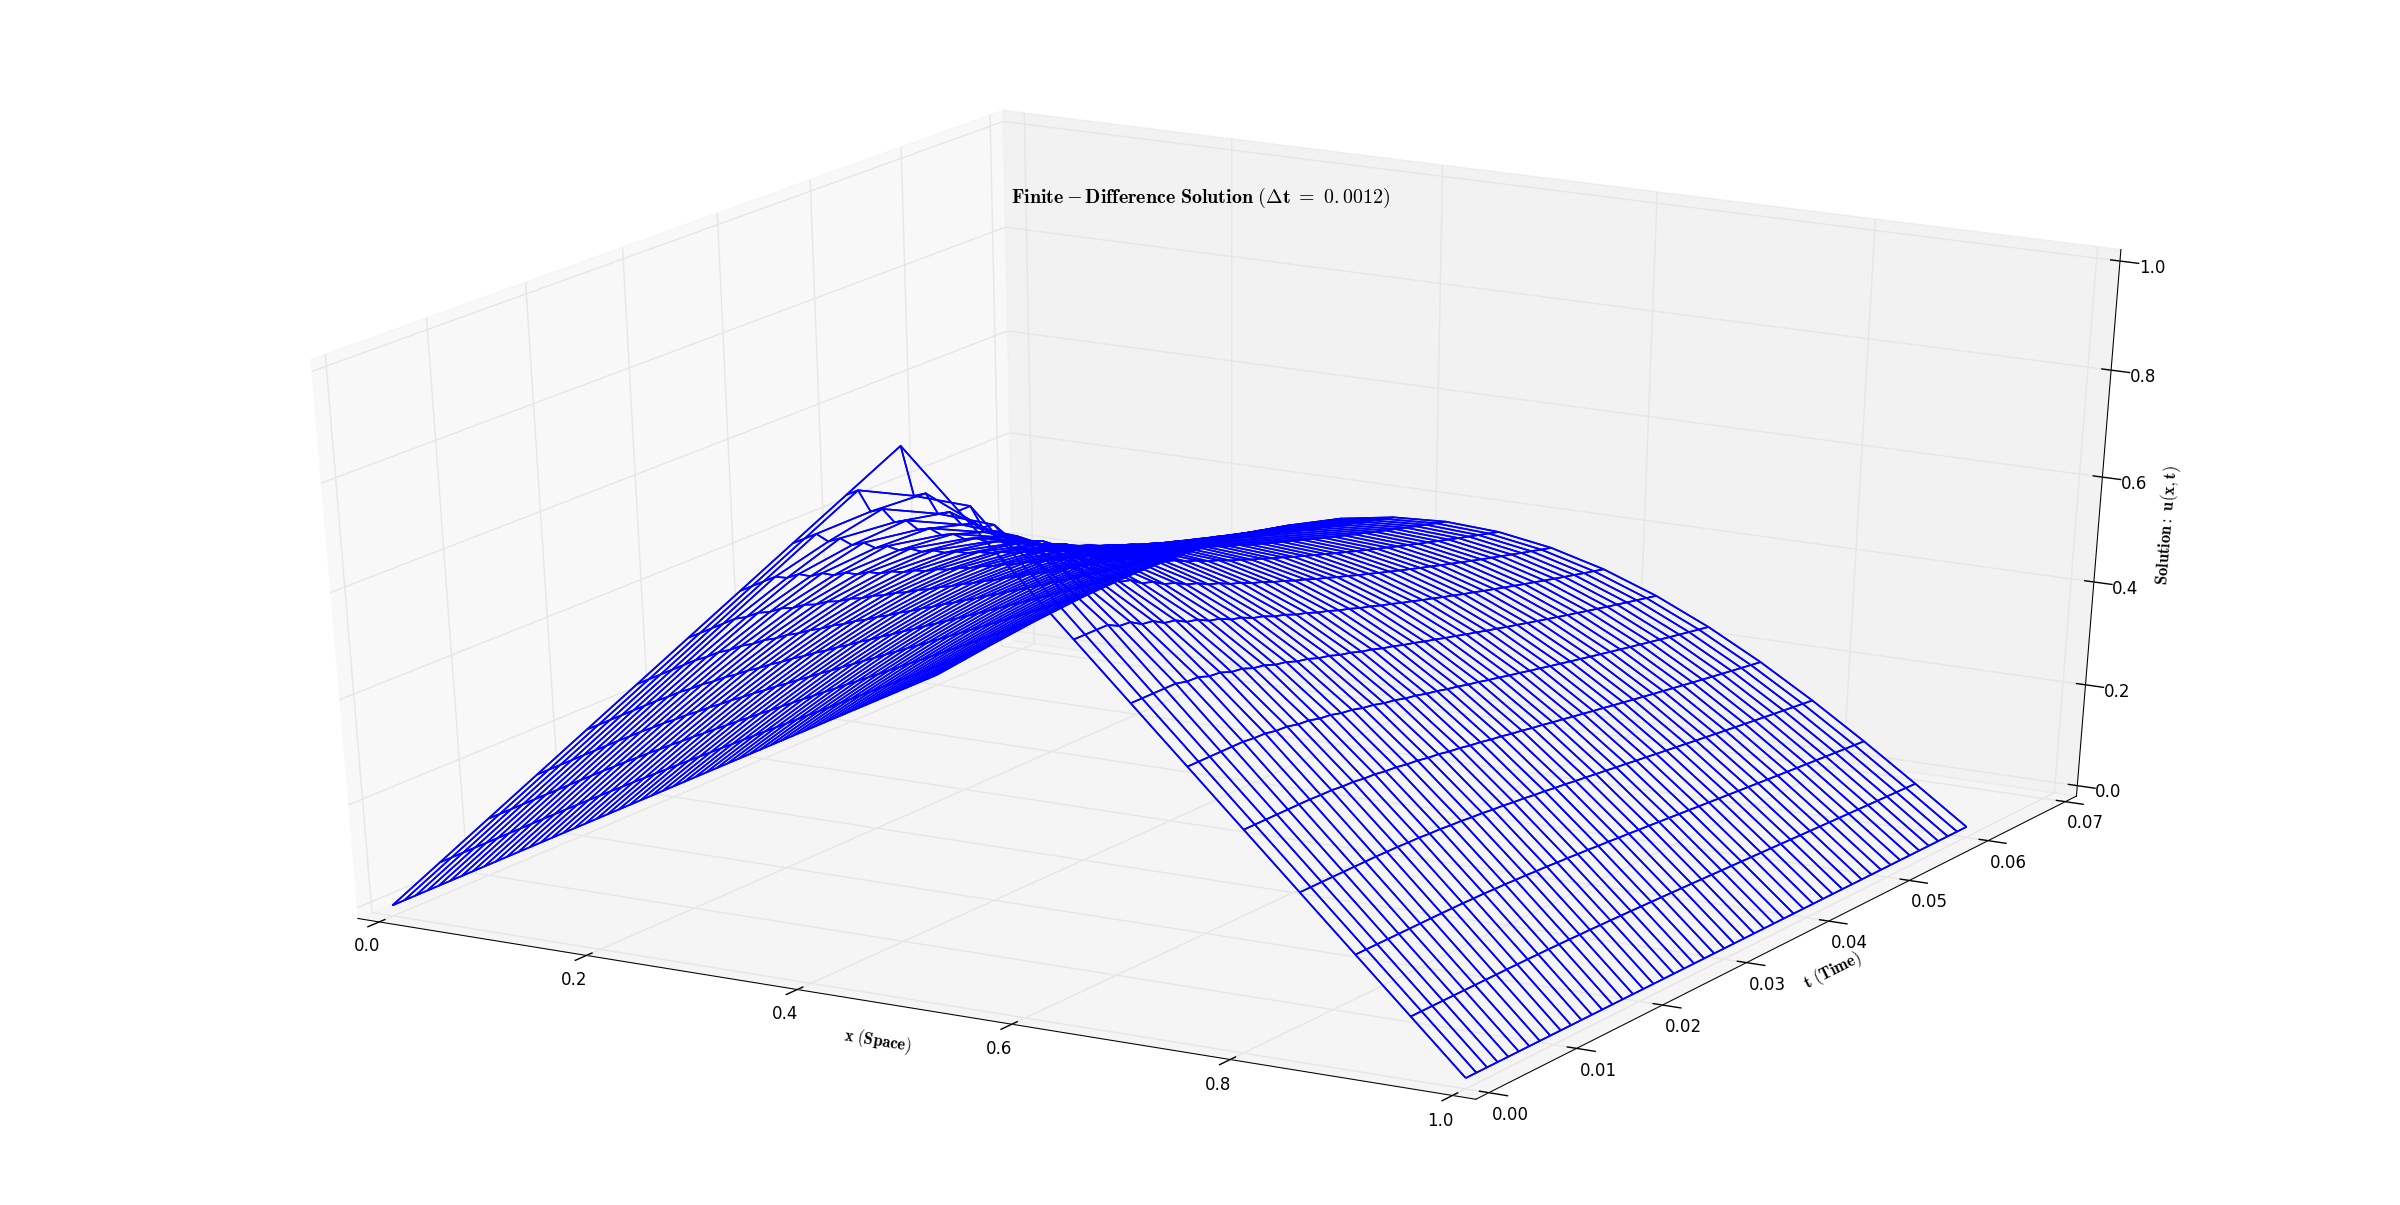
\includegraphics[width=7in, height=4.2in]{Fig1}
\caption{Forward-Time-Centered-Space (FTCS) Method or Euler's method }
\end{figure}
\begin{figure}[H]
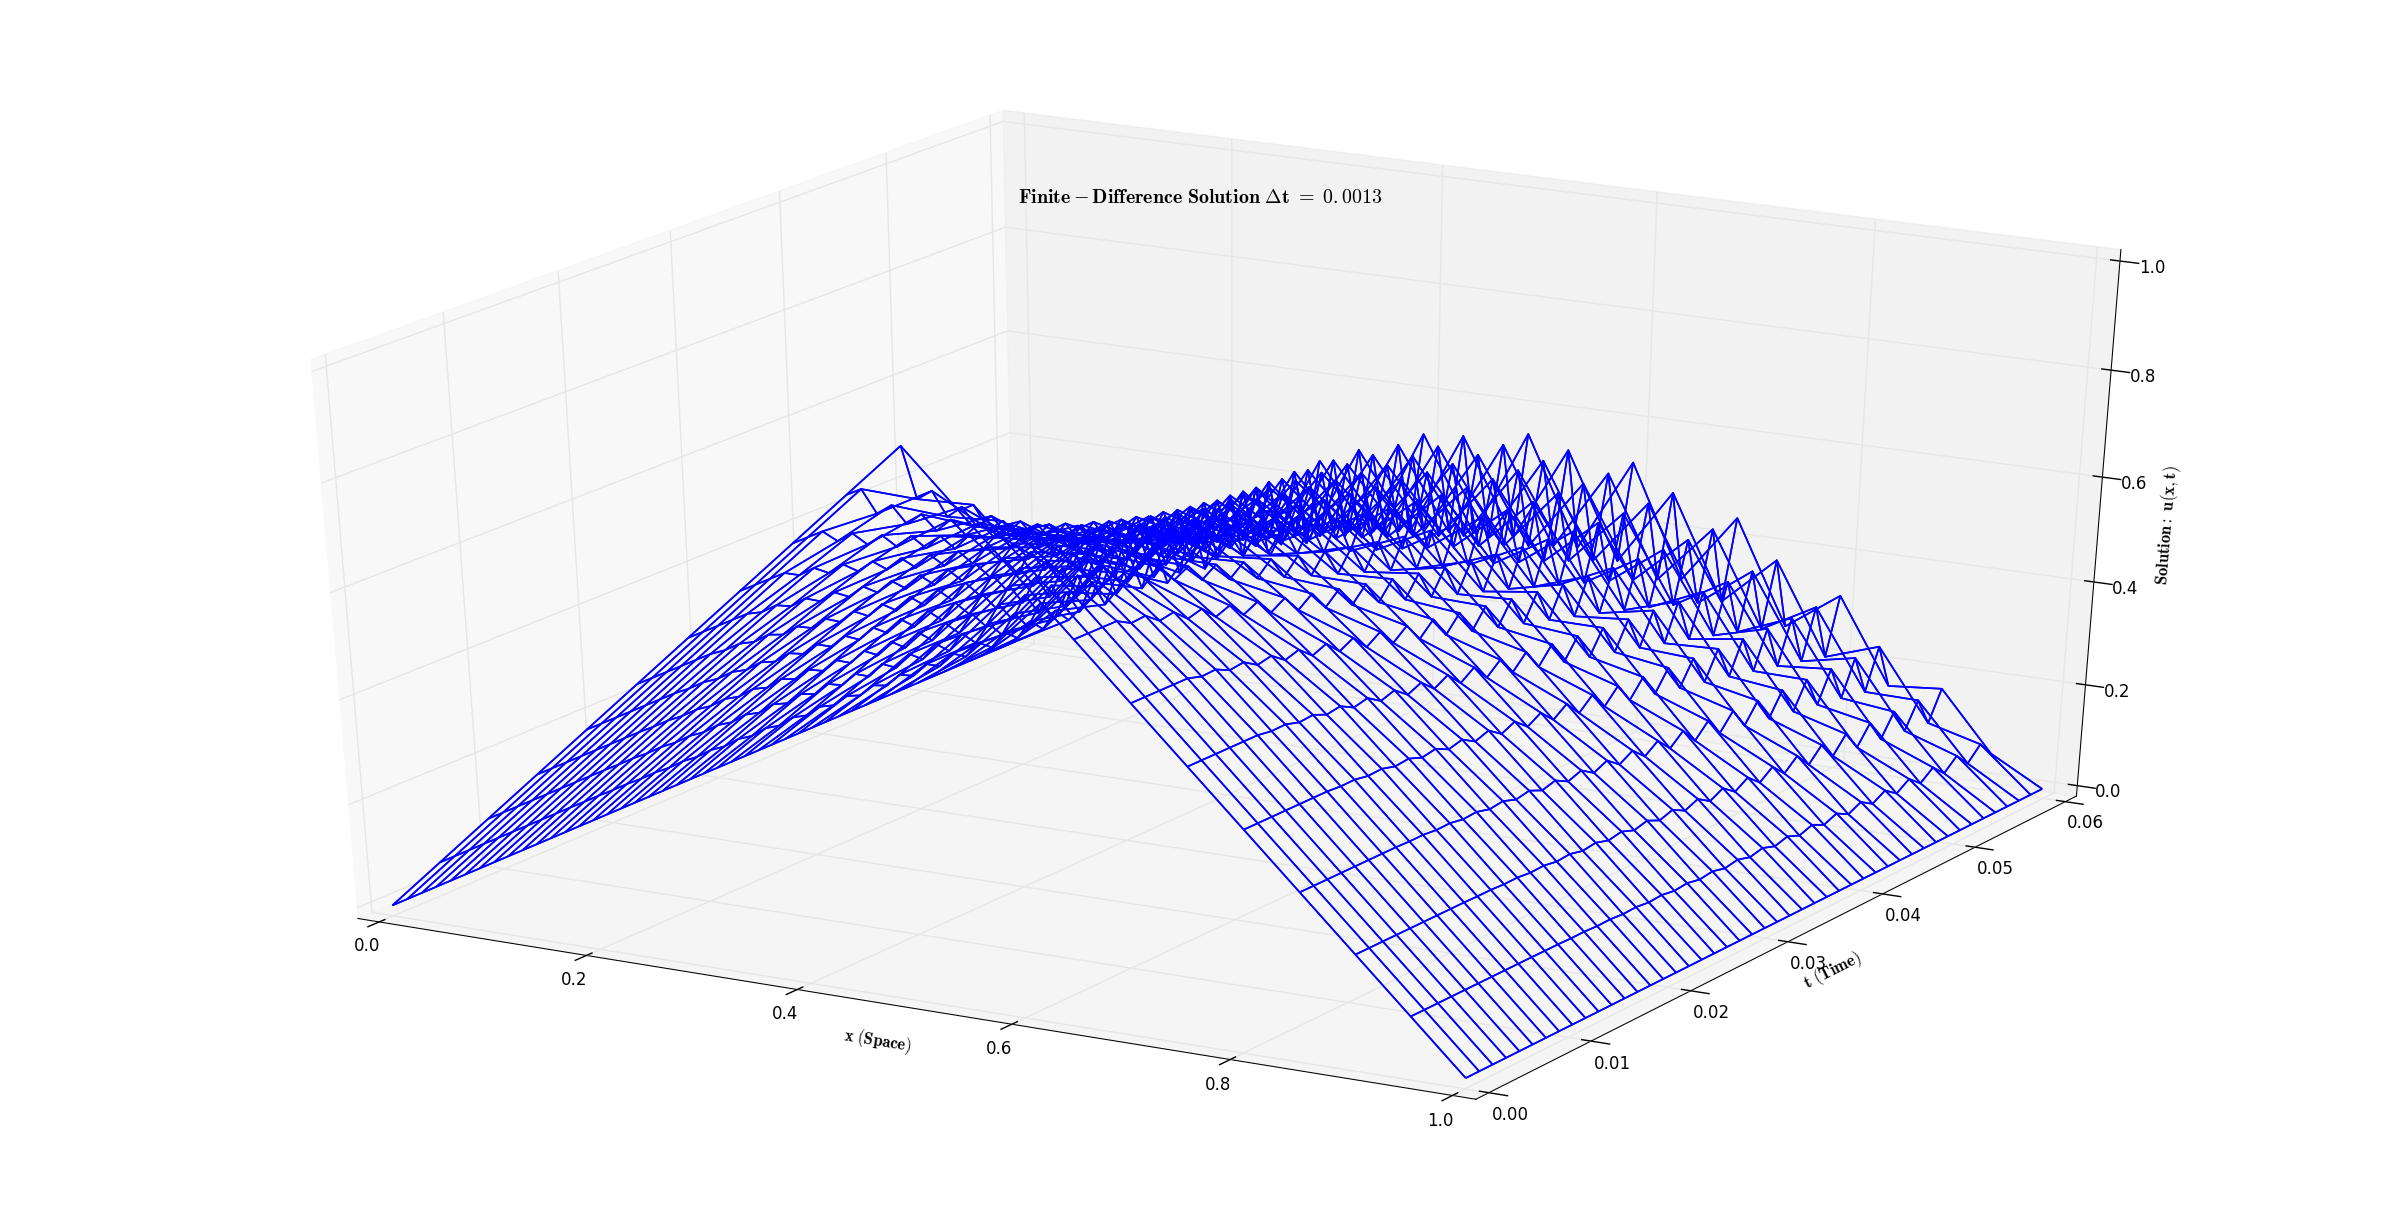
\includegraphics[width=7in, height=4.5in]{Fig2}
\caption{Forward-Time-Centered-Space (FTCS) Discretization - Coarser Step }
\end{figure}
\item The second plot has a coarser step size, i.e. $\Delta t_2 > \Delta t_1$, and for an explicit Finite-Difference-Discretization, {\bf the stability of the solution (which in this case can be shown to be unstable) decreases as we increase the step size}. 
\item Moreover this is evident by the fluctuations (spikes) towards the end of the time axis. Thus {\bf increasing the step-size decreases the stability of the solution}.
\item The stability of the Euler's method is ensured by the inequality 
\begin{align*}
\Delta t \leq \frac{{(\Delta x)}^2}{2c}
\end{align*}
But in our case we have
\begin{align*}
\Delta t = 0.0013\ \ ; \ \ \ \ \frac{{(\Delta x)}^2}{2c} = 1.25\ {\rm x}\ 10^{-3} \ \ ; \ \ \ \ \Delta t \nless \frac{{(\Delta x)}^2}{2c} 
\end{align*}
\item Hence the explicit scheme in the second case, $\Delta t = 0.0013$,is not stable whereas the one in the first case, $\Delta t = 0.0012$ is stable. 
\end{itemize}\hrule\newpage
\begin{itemize} 
\item The third plot corresponds to an implicit Finite-Difference-Discretization. The implicit method,is unconditionally stable, and hence stays stable even for the coarser step. 
\item The implicit method involves, for one space dimension, involves {\bf solving a tridiagonal linear system} at each step. Hence, by construction, it is unconditionally stable for coarser (step) sizes in time. This is reflected by the third and fourth plots given below. 
\item The {\bf Backward Euler Method is first order accurate in time and second order in space.} 
\begin{figure}[H]
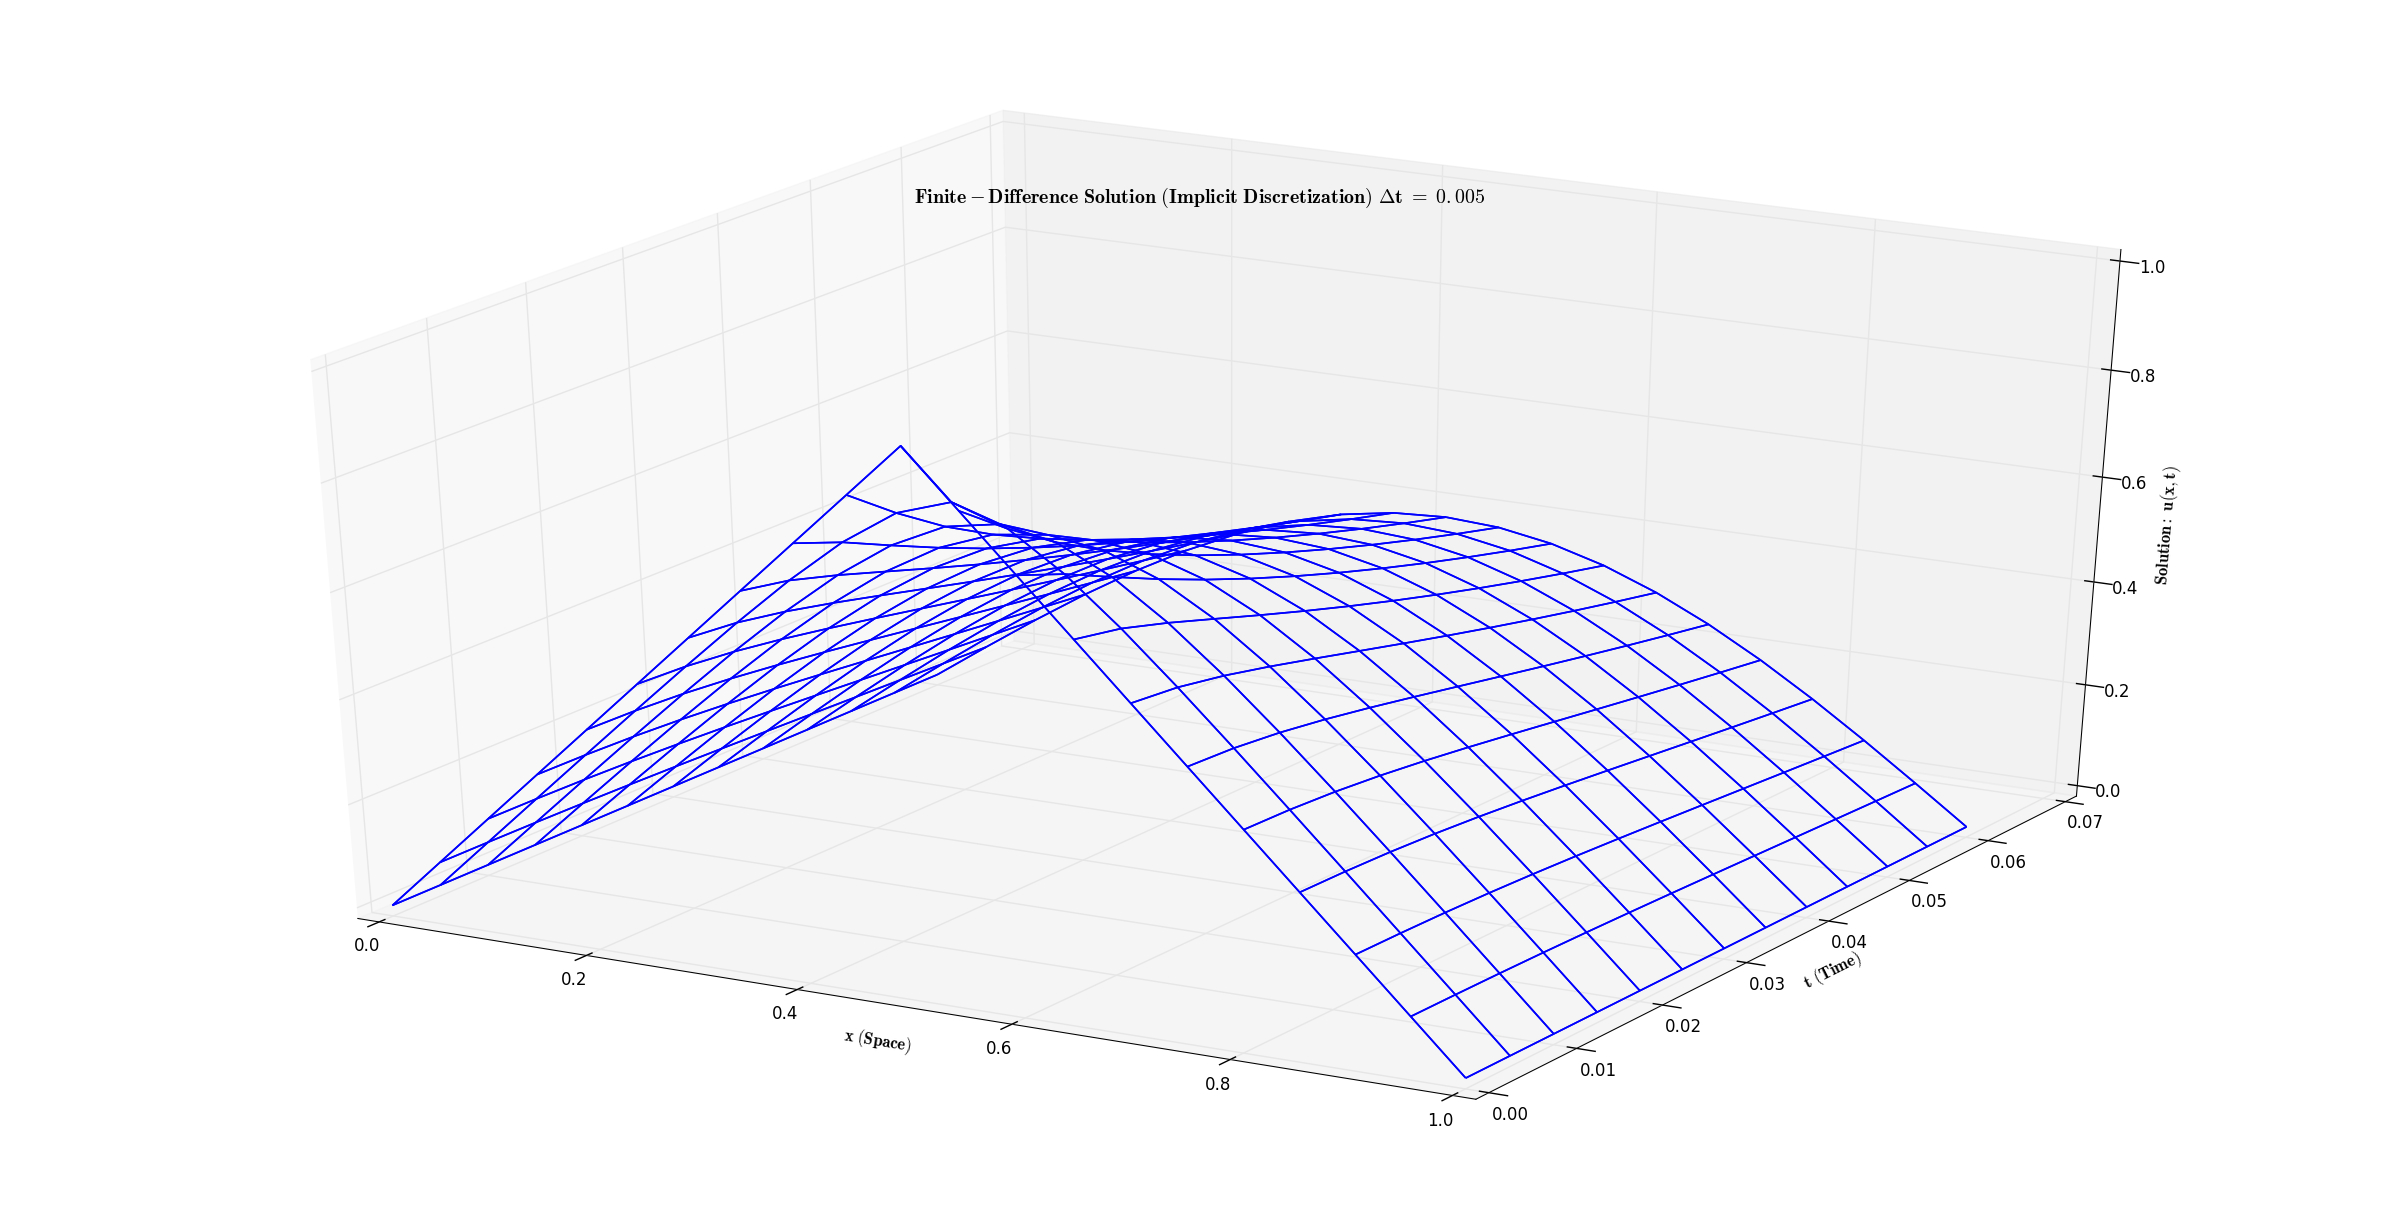
\includegraphics[width=7in, height=4.5in]{Fig3}
\caption{Backward-Time-Centered-Space (BTCS) or Backward Euler (Implicit FDM) }
\end{figure}\hrule
\newpage\item {\bf  The Crank-Nicolson method } 
\begin{figure}[H]
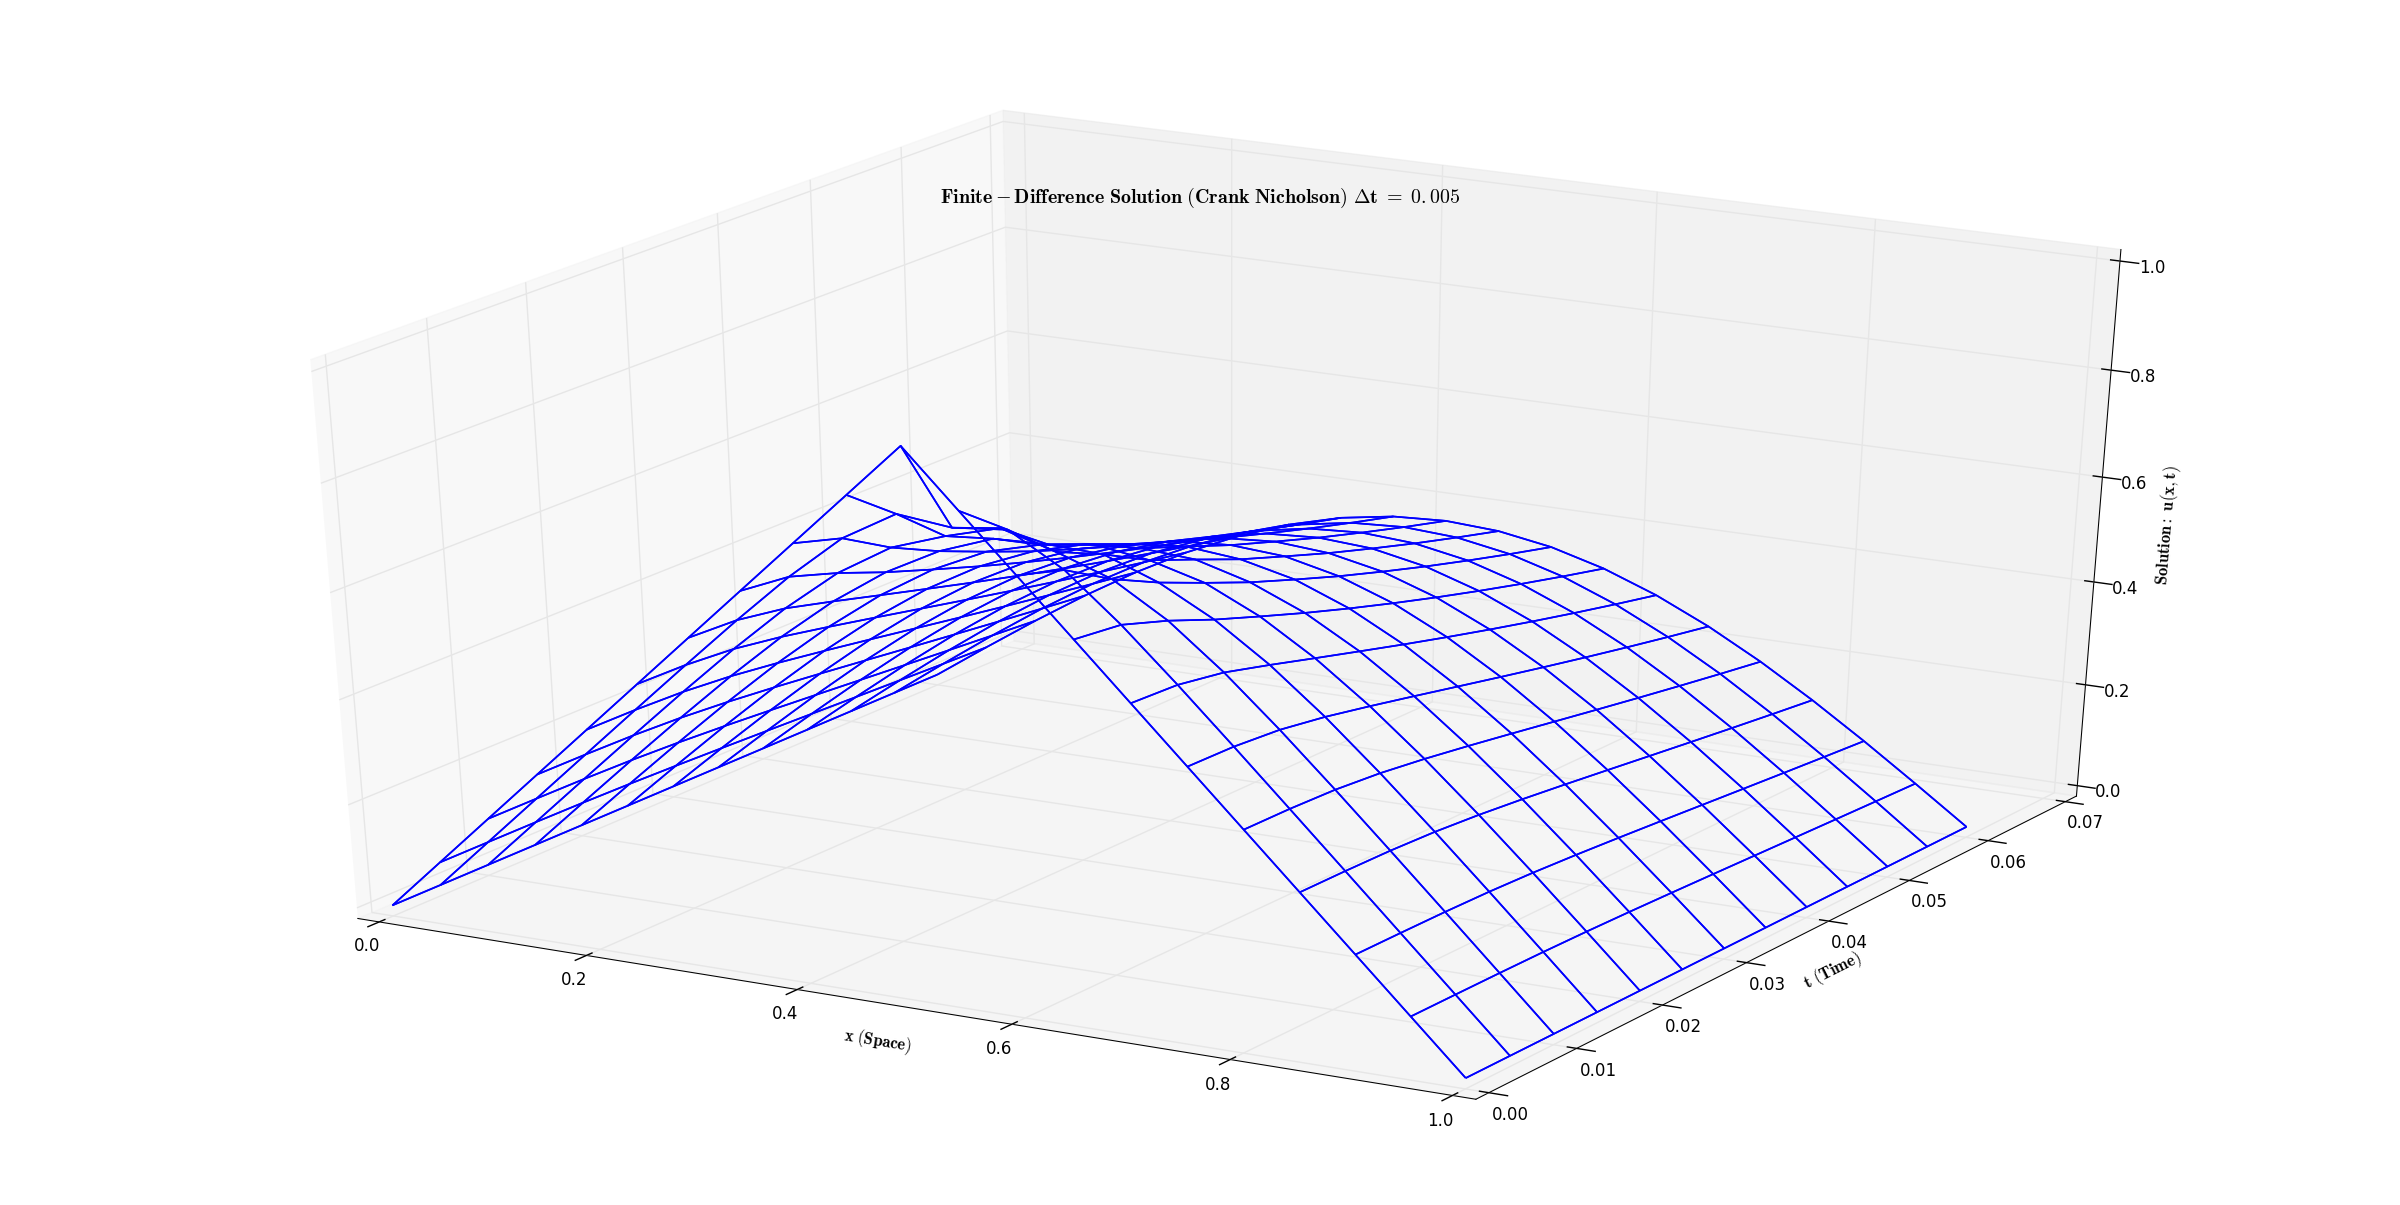
\includegraphics[width=7in, height=4.5in]{Fig4}
\caption{Crank Nicolson Discretization }
\end{figure}
\item The Crank-Nicolson method is more stable than the first two cases (due to its unconditional stability). 
\item There are small numerical errors, in case of Crank-Nicolson, as can be seen from the plot, (it crosses the z-axis at several places, though very slightly) which make it slightly less accurate than Backward-Euler. 
\item { \bf The Crank Nicolson method is second order accurate in both time and space, and hence more accurate than Backward Euler}
\item The Crank-Nicolson method is a combination of the Forward and Backward Euler methods. Hence, for the coarser step that we have considered, there is a small irregularity (non-smoothness) in the solution in the first step.  
\end{itemize}\hrule
\newpage
\begin{itemize}
\item The fifth plot corresponds to the semi-discrete method. The plot differs from the previous plots in the step size employed to solve the system. Since a library routine is used to solve the system of linear ODEs that result from the semi-discrete form, the time step is chosen automatically by the library routine \emph{scipy.integrate.odeint}. 
\item {\bf The Semi-Discrete method results in a stiff ODE system.}
\item The solution obtained from the Semi-Discrete Method is more stable than the explicit (Euler) method, however there is no considerable difference between the performance of the implicit methods (Backward-Euler and Crank-Nicolson).
\begin{figure}[H]
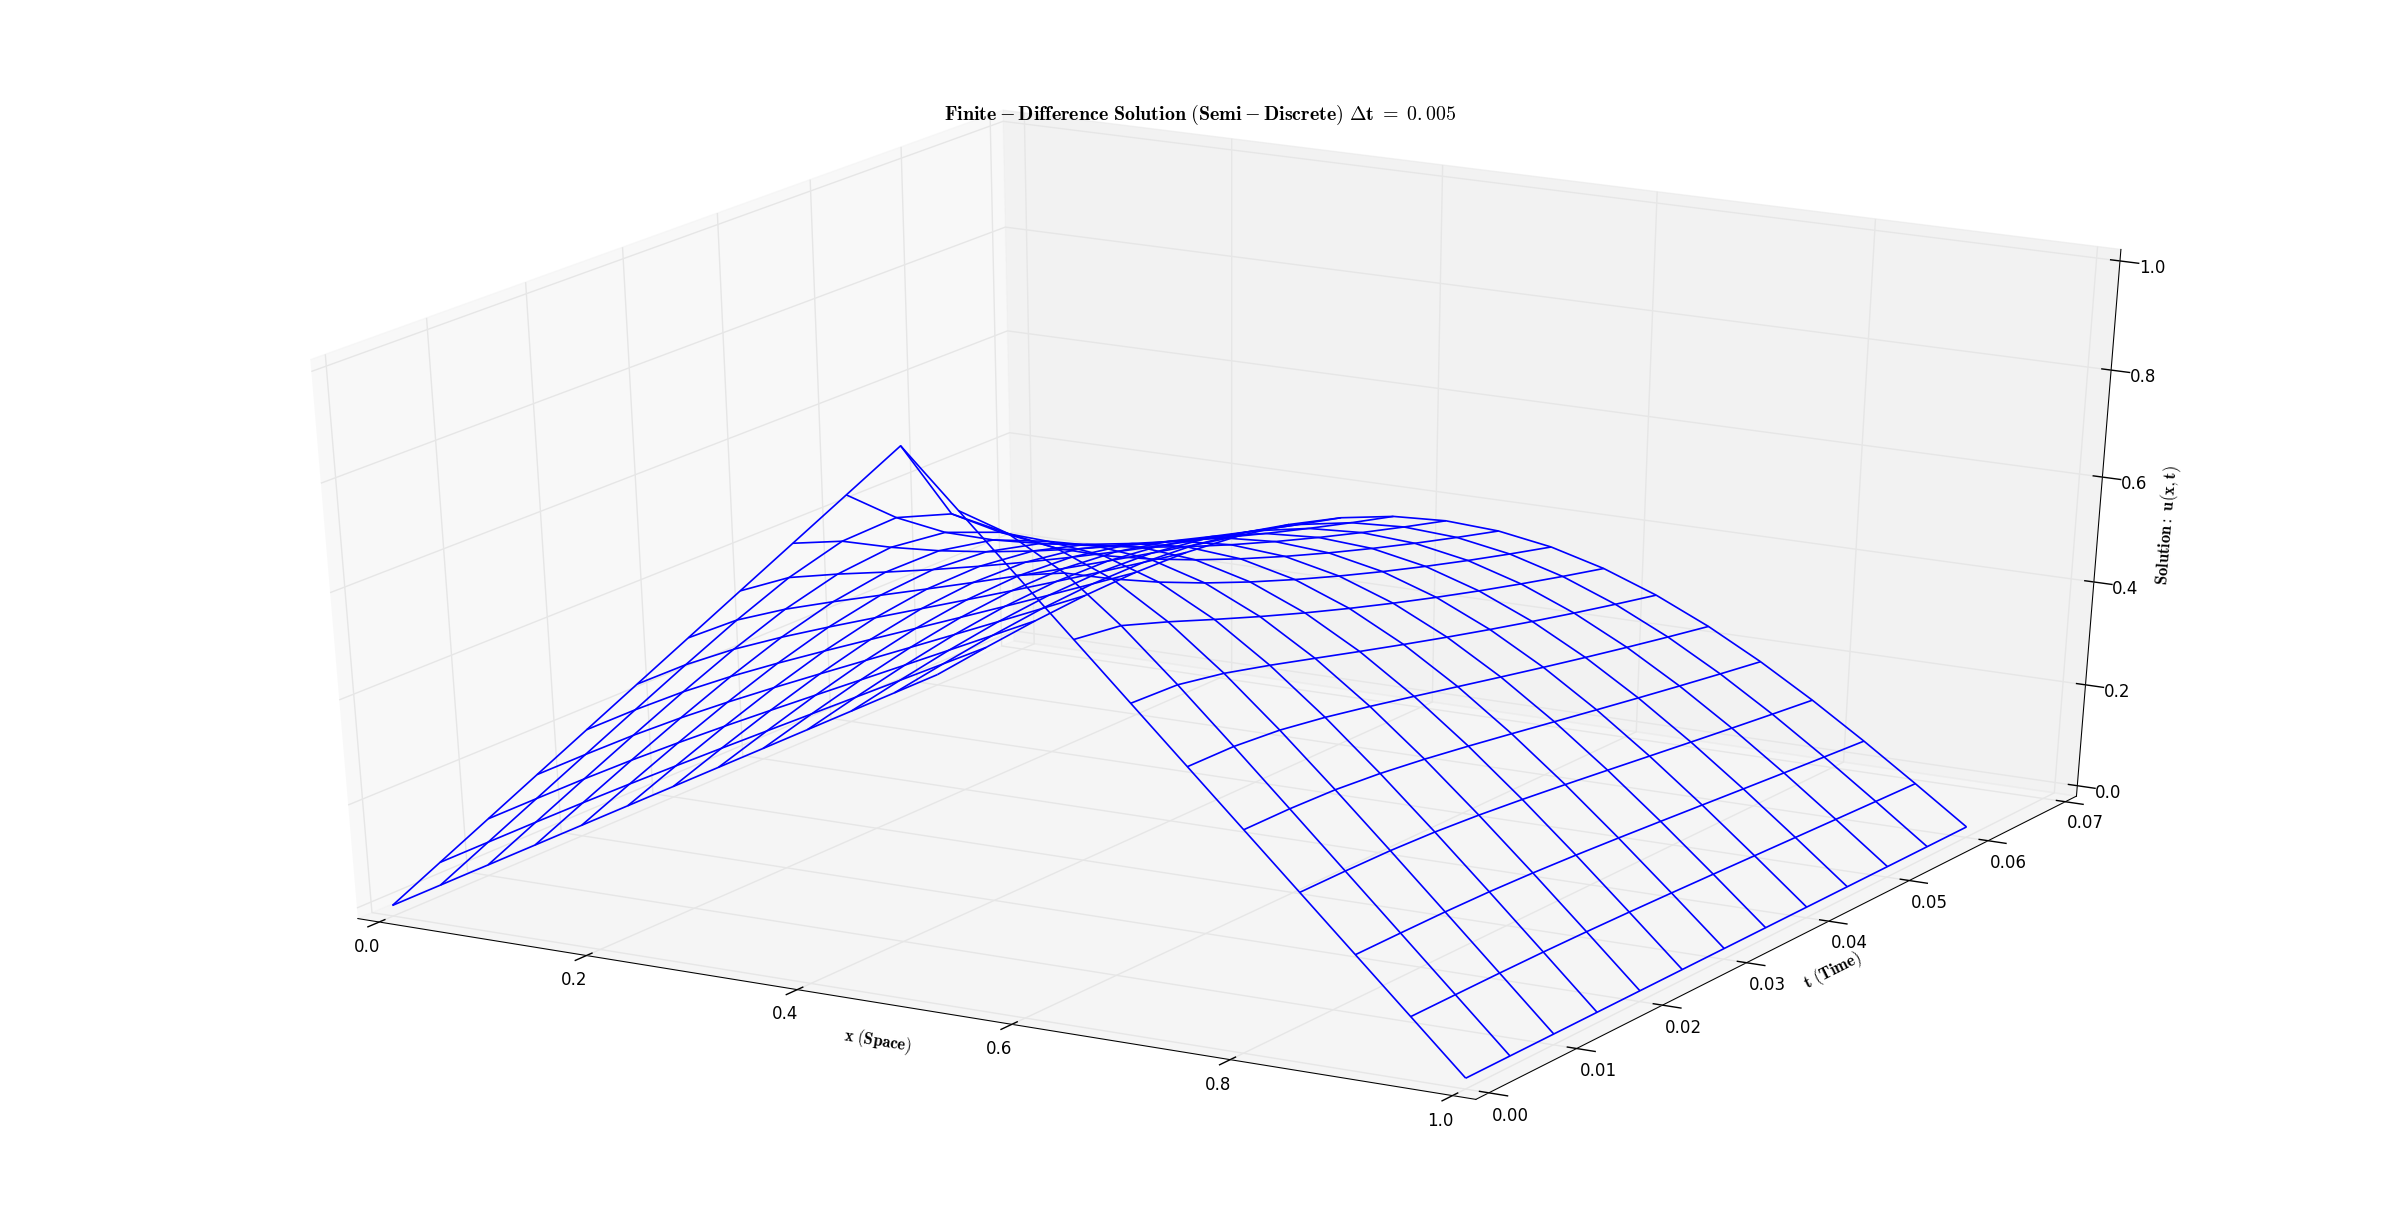
\includegraphics[width=7in, height=5in]{Fig5}
\caption{Semi-Discrete Method }
\end{figure}
\end{itemize}\hrule\hrule\hrule
\end{document}